%%%%%%%%%%%%%%%%%%%%%%%%%%%%%%%%%%%%%%%%%%%%%%%%%%%%%%%%%%%%%%%%%%%%%%%%%%%%%%%%%%%%%%%%%%%%%%%%%%%%%%%%%%%%%%%%%%%%%%%%%%%%%%%%%%%%%%%%%%%%%%%%%%%%%%%%%%%%%%%%%%%
% Written By Michael Brodskiy
% Class: Thermodynamics & Statistical Mechanics
% Professor: A. Stepanyants
%%%%%%%%%%%%%%%%%%%%%%%%%%%%%%%%%%%%%%%%%%%%%%%%%%%%%%%%%%%%%%%%%%%%%%%%%%%%%%%%%%%%%%%%%%%%%%%%%%%%%%%%%%%%%%%%%%%%%%%%%%%%%%%%%%%%%%%%%%%%%%%%%%%%%%%%%%%%%%%%%%%

\include{Includes.tex}

\title{Homework 7}
\date{November 15, 2023}
\author{Michael Brodskiy\\ \small Professor: A. Stepanyants}

\begin{document}

\maketitle

\begin{enumerate}

  \item

    \begin{enumerate}

      \item 

        First and foremost, we know:

        $$Q_h=Q_l+W$$
        $$W=Q_l-Q_h$$

        Per reversible conditions:

        $$\sigma_h=\sigma_l$$
        $$\frac{Q_h}{\tau_h}=\frac{Q_l}{\tau_l}$$
        $$Q_h=\frac{\tau_hQ_l}{\tau_l}$$

        Thus, we can combine to write:

        $$W=Q_h-\frac{\tau_l}{\tau_h}Q_h$$
        $$W=Q_h\left( 1-\frac{\tau_l}{\tau_h}\right)$$
        $$W=Q_h\left( \frac{\tau_h-\tau_l}{\tau_h}\right)$$

        And finally:

        $$\boxed{\frac{W}{Q_h}=\frac{\tau_h-\tau_l}{\tau_h}}$$

        If the heat pump is not reversible, we know the efficiency is:

        $$\frac{W}{Q_h}<\frac{\tau_h-\tau_l}{\tau_h}$$

      \item 

        We can write:

        $$W=(\tau_{hh}-\tau_l)\left( \frac{Q_{hh}}{\tau_{hh}}-\frac{Q_l}{\tau_l} \right)$$

        We know that the work generated is used as $Q_h$ in the heat pump:

        $$Q_h=(\tau_{hh}-\tau_l)\left( \frac{Q_{hh}}{\tau_{hh}}-\frac{Q_l}{\tau_l} \right)$$

        We can then rearrange to find the desired ratio:

        $$\frac{Q_h}{\tau_{hh}-\tau_l}=\frac{Q_{hh}\tau_l-Q_l\tau_{hh}}{\tau_{hh}\tau_l}$$
        $$\frac{\tau_{hh}\tau_l}{\tau_{hh}-\tau_l}=\frac{Q_{hh}\tau_l-Q_l\tau_{hh}}{Q_h}$$

        We know $Q_l=\frac{\tau_l}{\tau_h}Q_h$, which gives us:

        $$\frac{\tau_{hh}\tau_l}{\tau_{hh}-\tau_l}=\frac{Q_{hh}\tau_l}{Q_h}-\frac{\tau_l\tau_{hh}}{\tau_h}$$
        $$\boxed{\frac{Q_{hh}}{Q_h}=\frac{\tau_{hh}}{\tau_{hh}-\tau_l}+\frac{\tau_{hh}}{\tau_h}}$$

        Using the given values, we obtain:

        $$\frac{Q_{hh}}{Q_h}=\frac{600}{600-270}+2$$
        $$\boxed{\frac{Q_{hh}}{Q_h}=3.82}$$

      \item 

        For this problem, we essentially need to draw a ``double Carnot engine,'' with the output work of one ($W$) being the $Q_h$ of the second:

        \begin{figure}[H]
          \centering
          \tikzset{every picture/.style={line width=0.75pt}} %set default line width to 0.75pt        

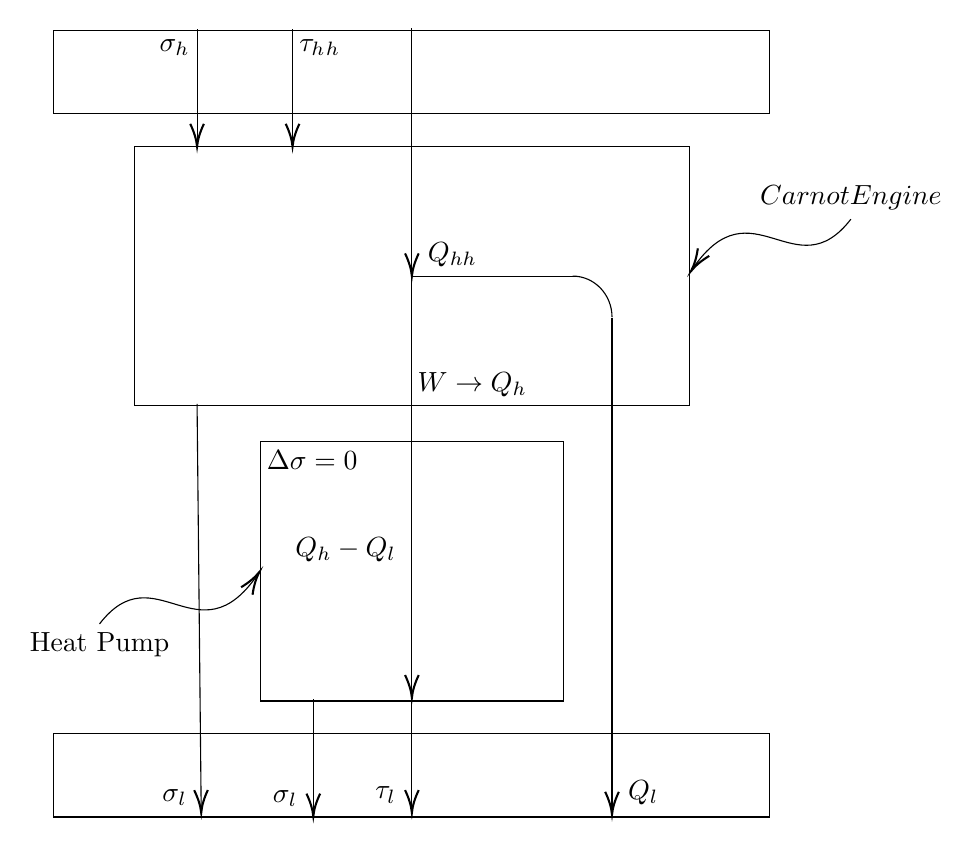
\begin{tikzpicture}[x=0.75pt,y=0.75pt,yscale=-1,xscale=1]
%uncomment if require: \path (0,444); %set diagram left start at 0, and has height of 444

%Shape: Rectangle [id:dp10170211024317433] 
\draw   (147,21) -- (492,21) -- (492,61) -- (147,61) -- cycle ;
%Shape: Rectangle [id:dp4544811596066871] 
\draw   (147,360) -- (492,360) -- (492,400) -- (147,400) -- cycle ;
%Shape: Rectangle [id:dp3842791172068818] 
\draw   (185.75,76.88) -- (453.25,76.88) -- (453.25,201.96) -- (185.75,201.96) -- cycle ;
%Shape: Rectangle [id:dp8874129257814114] 
\draw   (246.38,219.04) -- (392.63,219.04) -- (392.63,344.12) -- (246.38,344.12) -- cycle ;
%Curve Lines [id:da12079388453509687] 
\draw    (531,112) .. controls (504.27,146.65) and (483.42,94.07) .. (454.87,135.71) ;
\draw [shift={(454,137)}, rotate = 303.39] [color={rgb, 255:red, 0; green, 0; blue, 0 }  ][line width=0.75]    (10.93,-3.29) .. controls (6.95,-1.4) and (3.31,-0.3) .. (0,0) .. controls (3.31,0.3) and (6.95,1.4) .. (10.93,3.29)   ;
%Straight Lines [id:da13771774514472246] 
\draw    (319.5,20) -- (319.5,137.42) ;
\draw [shift={(319.5,139.42)}, rotate = 270] [color={rgb, 255:red, 0; green, 0; blue, 0 }  ][line width=0.75]    (10.93,-3.29) .. controls (6.95,-1.4) and (3.31,-0.3) .. (0,0) .. controls (3.31,0.3) and (6.95,1.4) .. (10.93,3.29)   ;
%Straight Lines [id:da42095144155513076] 
\draw    (319.5,139.42) -- (319.5,340.58) ;
\draw [shift={(319.5,342.58)}, rotate = 270] [color={rgb, 255:red, 0; green, 0; blue, 0 }  ][line width=0.75]    (10.93,-3.29) .. controls (6.95,-1.4) and (3.31,-0.3) .. (0,0) .. controls (3.31,0.3) and (6.95,1.4) .. (10.93,3.29)   ;
%Straight Lines [id:da693914432473546] 
\draw    (415.92,159.42) -- (415.92,396.84) ;
\draw [shift={(415.92,398.84)}, rotate = 270] [color={rgb, 255:red, 0; green, 0; blue, 0 }  ][line width=0.75]    (10.93,-3.29) .. controls (6.95,-1.4) and (3.31,-0.3) .. (0,0) .. controls (3.31,0.3) and (6.95,1.4) .. (10.93,3.29)   ;
%Straight Lines [id:da18101276066233973] 
\draw    (397.92,139.42) -- (319.5,139.42) ;
%Straight Lines [id:da8566525074884959] 
\draw    (216,20.58) -- (216,75) ;
\draw [shift={(216,77)}, rotate = 270] [color={rgb, 255:red, 0; green, 0; blue, 0 }  ][line width=0.75]    (10.93,-3.29) .. controls (6.95,-1.4) and (3.31,-0.3) .. (0,0) .. controls (3.31,0.3) and (6.95,1.4) .. (10.93,3.29)   ;
%Straight Lines [id:da2421143339083962] 
\draw    (272,343.29) -- (272,397.71) ;
\draw [shift={(272,399.71)}, rotate = 270] [color={rgb, 255:red, 0; green, 0; blue, 0 }  ][line width=0.75]    (10.93,-3.29) .. controls (6.95,-1.4) and (3.31,-0.3) .. (0,0) .. controls (3.31,0.3) and (6.95,1.4) .. (10.93,3.29)   ;
%Straight Lines [id:da6170237872934388] 
\draw    (319.5,342.58) -- (319.5,396) ;
\draw [shift={(319.5,398)}, rotate = 270] [color={rgb, 255:red, 0; green, 0; blue, 0 }  ][line width=0.75]    (10.93,-3.29) .. controls (6.95,-1.4) and (3.31,-0.3) .. (0,0) .. controls (3.31,0.3) and (6.95,1.4) .. (10.93,3.29)   ;
%Straight Lines [id:da3109235268228321] 
\draw    (262,20.58) -- (262,75) ;
\draw [shift={(262,77)}, rotate = 270] [color={rgb, 255:red, 0; green, 0; blue, 0 }  ][line width=0.75]    (10.93,-3.29) .. controls (6.95,-1.4) and (3.31,-0.3) .. (0,0) .. controls (3.31,0.3) and (6.95,1.4) .. (10.93,3.29)   ;
%Shape: Arc [id:dp5226403073336301] 
\draw  [draw opacity=0] (396.94,139.42) .. controls (396.94,139.42) and (396.94,139.42) .. (396.94,139.42) .. controls (396.94,139.42) and (396.94,139.42) .. (396.94,139.42) .. controls (407.42,139.42) and (415.92,148.28) .. (415.92,159.21) -- (396.94,159.21) -- cycle ; \draw   (396.94,139.42) .. controls (396.94,139.42) and (396.94,139.42) .. (396.94,139.42) .. controls (396.94,139.42) and (396.94,139.42) .. (396.94,139.42) .. controls (407.42,139.42) and (415.92,148.28) .. (415.92,159.21) ;  
%Curve Lines [id:da04778616308795569] 
\draw    (169,307) .. controls (195.73,272.35) and (216.58,324.93) .. (245.13,283.29) ;
\draw [shift={(246,282)}, rotate = 123.39] [color={rgb, 255:red, 0; green, 0; blue, 0 }  ][line width=0.75]    (10.93,-3.29) .. controls (6.95,-1.4) and (3.31,-0.3) .. (0,0) .. controls (3.31,0.3) and (6.95,1.4) .. (10.93,3.29)   ;
%Straight Lines [id:da8681702403313141] 
\draw    (216,201) -- (217.98,396) ;
\draw [shift={(218,398)}, rotate = 269.42] [color={rgb, 255:red, 0; green, 0; blue, 0 }  ][line width=0.75]    (10.93,-3.29) .. controls (6.95,-1.4) and (3.31,-0.3) .. (0,0) .. controls (3.31,0.3) and (6.95,1.4) .. (10.93,3.29)   ;

% Text Node
\draw (213.75,24.28) node [anchor=north east] [inner sep=0.75pt]    {$\sigma _{h}$};
% Text Node
\draw (264,23.98) node [anchor=north west][inner sep=0.75pt]    {$\tau _{h}{}_{h}$};
% Text Node
\draw (216.75,395.9) node [anchor=south east] [inner sep=0.75pt]    {$\sigma _{l} \ $};
% Text Node
\draw (321.5,136.02) node [anchor=south west] [inner sep=0.75pt]    {$\ Q_{hh}$};
% Text Node
\draw (417.92,395.44) node [anchor=south west] [inner sep=0.75pt]    {$\ Q_{l}$};
% Text Node
\draw (321,198.71) node [anchor=south west] [inner sep=0.75pt]    {$W\rightarrow Q_{h}$};
% Text Node
\draw (270,396.31) node [anchor=south east] [inner sep=0.75pt]    {$\sigma _{l} \ $};
% Text Node
\draw (317.5,278.18) node [anchor=south east] [inner sep=0.75pt]    {$Q_{h} -Q_{l} \ $};
% Text Node
\draw (317.5,394.6) node [anchor=south east] [inner sep=0.75pt]    {$\tau _{l} \ $};
% Text Node
\draw (248.38,222.44) node [anchor=north west][inner sep=0.75pt]    {$\Delta \sigma =0$};
% Text Node
\draw (531,108.6) node [anchor=south] [inner sep=0.75pt]    {$\text{Carnot Engine}$};
% Text Node
\draw (169,310) node [anchor=north] [inner sep=0.75pt]   [align=left] {Heat Pump};


\end{tikzpicture}

          \caption{Carnot Engine Feeding a Heat Pump}
          \label{fig:1}
        \end{figure}

    \end{enumerate}

  \item

    \begin{enumerate}

      \item 

        Similar to Figure \ref{fig:1}, we must have the pilot flame feed into the refrigerator:

        \begin{figure}[H]
          \centering
          \tikzset{every picture/.style={line width=0.75pt}} %set default line width to 0.75pt        

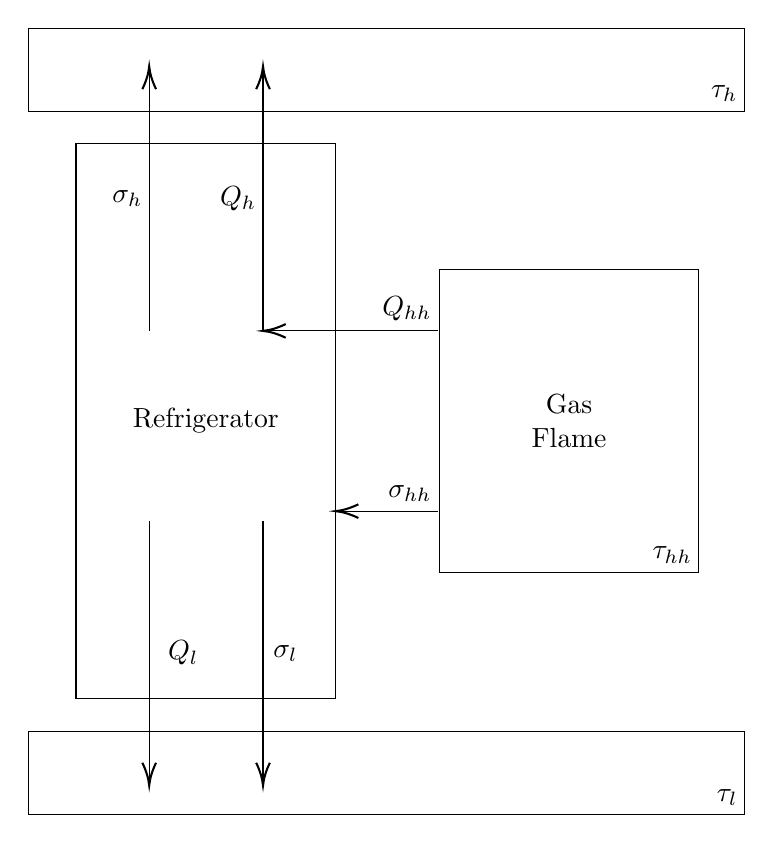
\begin{tikzpicture}[x=0.75pt,y=0.75pt,yscale=-1,xscale=1]
%uncomment if require: \path (0,444); %set diagram left start at 0, and has height of 444

%Shape: Rectangle [id:dp10170211024317433] 
\draw   (147,21) -- (492,21) -- (492,61) -- (147,61) -- cycle ;
%Shape: Rectangle [id:dp4544811596066871] 
\draw   (147,360) -- (492,360) -- (492,400) -- (147,400) -- cycle ;
%Shape: Rectangle [id:dp3842791172068818] 
\draw   (295.08,76.5) -- (295.08,344) -- (170,344) -- (170,76.5) -- cycle ;
%Shape: Rectangle [id:dp8874129257814114] 
\draw   (470.08,137.13) -- (470.08,283.38) -- (345,283.38) -- (345,137.13) -- cycle ;
%Straight Lines [id:da32858104289441736] 
\draw    (344.54,253.67) -- (297.12,253.67) ;
\draw [shift={(295.12,253.67)}, rotate = 360] [color={rgb, 255:red, 0; green, 0; blue, 0 }  ][line width=0.75]    (10.93,-3.29) .. controls (6.95,-1.4) and (3.31,-0.3) .. (0,0) .. controls (3.31,0.3) and (6.95,1.4) .. (10.93,3.29)   ;
%Straight Lines [id:da3165588536319903] 
\draw    (344.54,166.83) -- (262.12,166.83) ;
\draw [shift={(260.12,166.83)}, rotate = 360] [color={rgb, 255:red, 0; green, 0; blue, 0 }  ][line width=0.75]    (10.93,-3.29) .. controls (6.95,-1.4) and (3.31,-0.3) .. (0,0) .. controls (3.31,0.3) and (6.95,1.4) .. (10.93,3.29)   ;
%Straight Lines [id:da25070487209015857] 
\draw    (260.12,166.83) -- (260.12,41.41) ;
\draw [shift={(260.12,39.41)}, rotate = 90] [color={rgb, 255:red, 0; green, 0; blue, 0 }  ][line width=0.75]    (10.93,-3.29) .. controls (6.95,-1.4) and (3.31,-0.3) .. (0,0) .. controls (3.31,0.3) and (6.95,1.4) .. (10.93,3.29)   ;
%Straight Lines [id:da9292611993021886] 
\draw    (205.28,166.83) -- (205.28,41.41) ;
\draw [shift={(205.28,39.41)}, rotate = 90] [color={rgb, 255:red, 0; green, 0; blue, 0 }  ][line width=0.75]    (10.93,-3.29) .. controls (6.95,-1.4) and (3.31,-0.3) .. (0,0) .. controls (3.31,0.3) and (6.95,1.4) .. (10.93,3.29)   ;
%Straight Lines [id:da32161089218702354] 
\draw    (205.28,258.41) -- (205.28,383.83) ;
\draw [shift={(205.28,385.83)}, rotate = 270] [color={rgb, 255:red, 0; green, 0; blue, 0 }  ][line width=0.75]    (10.93,-3.29) .. controls (6.95,-1.4) and (3.31,-0.3) .. (0,0) .. controls (3.31,0.3) and (6.95,1.4) .. (10.93,3.29)   ;
%Straight Lines [id:da06444914845130922] 
\draw    (260.12,258.41) -- (260.12,383.83) ;
\draw [shift={(260.12,385.83)}, rotate = 270] [color={rgb, 255:red, 0; green, 0; blue, 0 }  ][line width=0.75]    (10.93,-3.29) .. controls (6.95,-1.4) and (3.31,-0.3) .. (0,0) .. controls (3.31,0.3) and (6.95,1.4) .. (10.93,3.29)   ;

% Text Node
\draw (490,57.6) node [anchor=south east] [inner sep=0.75pt]    {$\tau _{h}$};
% Text Node
\draw (490,396.6) node [anchor=south east] [inner sep=0.75pt]    {$\tau _{l}$};
% Text Node
\draw (468.08,279.97) node [anchor=south east] [inner sep=0.75pt]    {$\tau _{hh}$};
% Text Node
\draw (342.54,250.27) node [anchor=south east] [inner sep=0.75pt]    {$\sigma _{hh}$};
% Text Node
\draw (342.54,163.43) node [anchor=south east] [inner sep=0.75pt]    {$Q_{hh}$};
% Text Node
\draw (407.54,210.25) node   [align=left] {\begin{minipage}[lt]{31.07pt}\setlength\topsep{0pt}
\begin{center}
Gas \\Flame
\end{center}

\end{minipage}};
% Text Node
\draw (258.12,103.12) node [anchor=east] [inner sep=0.75pt]    {$Q_{h}$};
% Text Node
\draw (203.28,103.12) node [anchor=east] [inner sep=0.75pt]    {$\sigma _{h}$};
% Text Node
\draw (230.28,322.12) node [anchor=east] [inner sep=0.75pt]    {$Q_{l}$};
% Text Node
\draw (278.12,322.12) node [anchor=east] [inner sep=0.75pt]    {$\sigma _{l}$};
% Text Node
\draw (232.54,210.25) node   [align=left] {Refrigerator};


\end{tikzpicture}

          \caption{Pilot Flame Feeding a Refrigerator}
          \label{fig:2}
        \end{figure}

      \item 

        First, we assume that this is a reversible refrigerator. This gives us:

        $$\frac{Q_{hh}}{\tau_{hh}}+\frac{Q_l}{\tau_l}-\frac{Q_h}{\tau_h}=0$$

        Furthermore, we know:

        $$Q_h=Q_l+Q_{hh}$$

        This gives us:

        $$\frac{Q_{hh}}{\tau_{hh}}+\frac{Q_l}{\tau_l}=\frac{Q_l+Q_{hh}}{\tau_h}$$

        We can rearrange:

        $$\frac{\tau_lQ_{hh}+Q_l\tau_{hh}}{\tau_l\tau_{hh}}=\frac{Q_l+Q_{hh}}{\tau_h}$$
        $$\tau_h(\tau_lQ_{hh}+Q_l\tau_{hh})=(Q_l+Q_{hh})(\tau_l\tau_{hh})$$
        $$\tau_h\tau_lQ_{hh}+Q_l\tau_{hh}\tau_h=\tau_l\tau_{hh}Q_l+\tau_l\tau_{hh}Q_{hh}$$

        We then separate $Q_{hh}$ and $Q_l$ to different sides:

        $$(\tau_h\tau_l-\tau_l\tau_{hh})Q_{hh}=(\tau_l\tau_{hh}-\tau_{hh}\tau_h)Q_l$$

        This then gives us:

        $$\boxed{\frac{Q_l}{Q_{hh}}=\frac{\tau_h\tau_l-\tau_l\tau_{hh}}{\tau_l\tau_{hh}-\tau_{hh}\tau_h}}$$

    \end{enumerate}

  \item

    \begin{enumerate}

      \item 

        The processes from stages $2\to3$ and $4\to1$ are both isentropic, indicating constant $\sigma$. This, in tandem with the fact that, for photons, $\sigma\propto V\tau^3$, allows us to write:

        $$V_2\tau_h^3=V_3\tau_l^3\quad\text{ and }\quad V_1\tau_h^3=V_4\tau_l^3$$
        $$\boxed{V_3=\left( \frac{\tau_h}{\tau_l} \right)^3V_2\quad\text{ and }\quad V_4=\left( \frac{\tau_h}{\tau_l} \right)^3V_1}$$
        
      \item 

        As with our ideal gas, we can derive the heat and work in a similar manner. First and foremost:

        $$Q_h=\tau_h\left( \sigma_2-\sigma_1\right)$$

        For a photon gas, we know:

        $$\sigma=\frac{4\pi^2V\tau^3}{45h^3c^3}$$

        This gives us:

        $$Q_h=\frac{4\pi^2\tau_h^4}{45h^3c^3}(V_2-V_1)$$

        Then, we need to employ the equation $Q_h=\Delta U+W$. We begin by finding $\Delta U$:

        $$U=\frac{\pi^2V\tau^4}{15h^3c^3}$$
        $$\Delta U=\frac{\pi^2\tau_h^4}{15h^3c^3}(V_2-V_1)$$

        We can see that the dependency on the volume makes it so that $\Delta U\neq0$, unlike an ideal gas. As such we may say that $\boxed{Q_h\neq W}$. We can also find the actual value of $W$ as:

        $$Q_h-\Delta U=\frac{\pi^2\tau_h^4}{45h^3c^3}(V_2-V_1)$$

        Thus, we can see:

        $$\boxed{\frac{4\pi^2\tau_h^4}{45h^3c^3}(V_2-V_1)\neq\frac{\pi^2\tau_h^4}{45h^3c^3}(V_2-V_1)}$$
        
      \item 

        For the isentropic processes, we know:

        $$Q=0$$

        This allows us to write:

        $$\Delta U+W=0$$
        $$W=-\Delta U$$

        For process $2\to3$, we may write:

        $$W=-(U_3-U_2)$$
        $$W=-\frac{\pi^2}{15h^3c^3}(V_3\tau_l^4-V_2\tau_h^4)$$

        For process $4\to1$, we may write:

        $$W=-(U_1-U_4)$$
        $$W=-\frac{\pi^2}{15h^3c^3}(V_1\tau_h^4-V_4\tau_l^4)$$

        Employing our results from part (a), we may write:

        $$W_{23}=-\frac{\pi^2}{15h^3c^3}(V_2\tau_l\tau_h^3-V_2\tau_h^4)$$
        $$W_{41}=-\frac{\pi^2}{15h^3c^3}(V_1\tau_h^4-V_1\tau_h^3\tau_l)$$

        These are equivalent to:

        $$W_{23}=\frac{\pi^2V_2\tau_h^3}{15h^3c^3}(\tau_h-\tau_l)$$
        $$W_{41}=\frac{\pi^2V_1\tau_h^3}{15h^3c^3}(\tau_l-\tau_h)$$

        Thus, we can see that, though similar, unlike an ideal gas, $\boxed{W_{23}\neq W_{41}}$
        
      \item 

        Using our results from (b) and (c), we can write:

        $$W_{12}=\frac{\pi^2\tau_h^4}{45h^3c^3}(V_2-V_1)$$
        $$W_{23}=\frac{\pi^2V_2\tau_h^3}{15h^3c^3}(\tau_h-\tau_l)$$
        $$W_{34}=\frac{\pi^2\tau_l^4}{45h^3c^3}(V_4-V_3)$$
        $$W_{41}=\frac{\pi^2V_1\tau_h^3}{15h^3c^3}(\tau_l-\tau_h)$$

        For $W_{34}$, we can employ the identities found in (a):

        $$W_{34}=\frac{\pi^2\tau_l\tau_h^3}{45h^3c^3}(V_1-V_2)$$

        Now, we can sum:

        $$W_{tot}=\frac{\pi^2\tau_h^4}{45h^3c^3}(V_2-V_1)+\frac{\pi^2V_2\tau_h^3}{15h^3c^3}(\tau_h-\tau_l)+\frac{\pi^2\tau_l\tau_h^3}{45h^3c^3}(V_1-V_2)+\frac{\pi^2V_1\tau_h^3}{15h^3c^3}(\tau_l-\tau_h)$$

        We can factor out the coefficients:

        $$W_{tot}=\frac{\pi^2\tau_h^3}{45h^3c^3}\left(\tau_h(V_2-V_1)+3V_2(\tau_h-\tau_l)+\tau_l(V_1-V_2)+3V_1(\tau_l-\tau_h)\right)$$

        We may continue by summing similar terms:

        $$W_{tot}=\frac{\pi^2\tau_h^3}{45h^3c^3}\left((\tau_h-\tau_l)(V_2-V_1)+3(V_2-V_1)(\tau_h-\tau_l)\right)$$

        Continuing simplification, we get:

        $$\boxed{W_{tot}=\frac{4\pi^2\tau_h^3}{45h^3c^3}(\tau_h-\tau_l)(V_2-V_1)}$$

        We know that the Carnot Energy efficiency formula may be expressed as:

        $$\eta_c=\frac{W_{tot}}{Q_{rec}}$$

        Dividing the above answer by the heat from part (b), we get:

        $$\boxed{\eta_c=\frac{(\tau_h-\tau_l)}{\tau_h}=\left( 1-\frac{\tau_l}{\tau_h} \right)}$$

        As can be seen, the efficiency formula remains the same
        
    \end{enumerate}

    \setcounter{enumi}{4}

  \item

    First and foremost, we may write:

    $$W=(\tau_h-\tau_l)\sigma_l$$

    Given the assumption that the process is reversible, we may write:

    $$\sigma_l=\frac{Q_l}{\tau_l}$$

    This gives us:

    $$W=\left( \frac{\tau_h}{\tau_l}-1 \right)Q_l$$

    We can apply the given parameters to find:

    $$W=\left( \frac{500}{20}-1 \right)1500$$
    $$\boxed{W=36[\si{\giga\watt}]}$$

    Given improvements, we can write:

    $$W=\left( \frac{600}{20}-1 \right)1500$$
    $$\boxed{W=43.5[\si{\giga\watt}]}$$

    Clearly, there is nearly a 20\% increase in the ability to produce energy

  \item

    \begin{enumerate}

      \item 

        First and foremost, we may write:

        $$W=\left( 1-\frac{\tau_l}{\tau_h} \right)Q_h=\left( \frac{\tau_h}{\tau_l}-1 \right)Q_l$$

        Given that:

        $$\frac{dW}{dt}=P$$

        We may obtain:

        $$P=\left( \frac{\tau_h}{\tau_l}-1 \right)\frac{dQ_l}{dt}$$

        From the problem, we may substitute:

        $$P=A\left( \frac{\tau_h}{\tau_l}-1 \right)(\tau_h-\tau_l)$$

        Multiplying both sides by $\tau_l$ and dividing by $A$, we get:

        $$\frac{P\tau_l}{A}=(\tau_h-\tau_l)^2$$
        $$\frac{P\tau_l}{A}=\tau_h^2-2\tau_h\tau_l+\tau_l^2$$

        We can then move all terms to one side:

        $$\frac{P\tau_l}{A}+2\tau_h\tau_l-\tau_l^2-\tau_h^2=0$$
        $$\left(\frac{P}{A}+2\tau_h\right)\tau_l-\tau_l^2-\tau_h^2=0$$

        Employing the quadratic equation, we obtain:

        $$\tau_l^2-\left( \frac{P}{A}+2\tau_h \right)\tau_l+\tau_h=0\to \left\{\begin{array}{l} a=1\\b=-\left( \frac{P}{A}+2\tau_h \right)\\c=\tau_h^2\end{array}$$
        $$\tau_l=\frac{1}{2}\left( \frac{P}{A}+2\tau_h-\sqrt{\left( \frac{P}{A}+2\tau_h \right)^2-4\tau_h^2}\right)$$

        Note: we can forego the solution with a positive determinant, as that would make $\tau_l>\tau_h$. Distributing, we finally obtain:

        $$\tau_l=\frac{P}{2A}+\tau_h-\left[ \left( \frac{P}{2A}+\tau_h \right)^2-\tau_h^2 \right]^{\frac{1}{2}}$$

        The Boltzmann factor cancels out, leaving us with:

        $$\boxed{T_l=\left(T_h+\frac{P}{2A}\right)-\left[ \left( T_h+\frac{P}{2A} \right)^2-T_h^2 \right]^{\frac{1}{2}}}$$

      \item 

        We can rearrange one of the formulas obtained in (a) to write:

        $$A=\frac{PT_l}{\left( T_h-T_l \right)^2}$$

        This gives us:

        $$A=\frac{(2\cdot10^3)(290)}{(20)^2}$$
        $$A=\frac{(580\cdot10^3)}{400}$$
        $$\boxed{A=1450\left[ \frac{\si{\watt}}{\si{\kelvin}} \right]}$$

    \end{enumerate}

  \item

    We know from (1) that:

    $$\frac{W}{Q_l}=\left( \frac{\tau_h}{\tau_l}-1 \right)$$

    And also that:

    $$W+Q_l=Q_h$$

    We can express the work done by the light bulb as $W=Q_l$. The total work of the two processes needs to equal zero, which allows us to write:

    $$\left( \frac{\tau_h}{\tau_l}-1 \right)Q_l-Q_l=0$$

    This simplifies to:

    $$\tau_h=2\tau_l$$

    Room temperature implies $27[\si{\celsius}]\to300[\si{\kelvin}]$

    Thus, the Carnot refrigerator, at peak efficiency, may cool to:

    $$\boxed{\tau_l=\frac{300}{2}=150[\si{\kelvin}]}$$

    Thus, the refrigerator should be able to cool below room temperature.

\end{enumerate}

\end{document}

